\documentclass{instructions}

\usepackage{xspace}

\newcommand\repo[1]{\url{https://github.com/severin-lemaignan/attention-assessment-workshop/#1}}
\newcommand\bs{\char`\\}

\venue{2nd HRI Summer School}
\title{From a video stream to attention assessment}
\date{August 25, 2015}

\summary{
Assessing in real-time the focus of attention of a human interacting with a
robot is essential to understand implicit references in a dialogue ("robot, take
that!"), to measure engagement (is the human "with me"?) or to detect outright
problems (why is this human staring at me since 20 minutes?)

With a regular camera, a bit of math and a good face detector, we can actually
estimate pretty accurately and in real-time the 3D head pose of surrounding
humans. Combined with some frames' magic, this lets us assess what the human is
looking at: his/her \emph{Visual Focus of Attention} or VFOA.

}

\objectives{
During the workshop, we will:

\begin{itemize}
    \item use a state-of-art open-source face detector (coming for the {\tt
        dlib} library) and
  a PnP algorithm (from OpenCV) to match a 3D template of a head onto a 2D
  camera stream,
  \item export the head pose as a ROS tf frame and visualize the face in RViz,
  \item write a dedicated ROS node that computes what is seen by the human at a given
  time,
  \item test the system in a pre-recorded scenario,
%  \item validate the approach by manually annotating the
%  focus of attention and computing an inter-judge agreement between the robot
%  and you (if time permits!).
\end{itemize}
}

\begin{document}

\maketitle

\intro

We will first make sure everything works well on your computer: {\tt dlib}, {\tt
opencv}, your compiler,... 

\note{This assumes, of course, that you have downloaded and
installed all the workshop's prerequisites. Otherwise, head to
\url{https://hrisummerschool15.wordpress.com/summer-school-programme/workshops/}
to get the list of prerequisites and quickly install them.
}

Go to \repo{} and download the repo as a zip file or clone it with {\tt git}.
Extract the content somewhere: this will be our \sh{$PROJECT_ROOT} directory.

Then recursively copy the content of {\tt templates/intro/} to the root
directory (\sh{$PROJECT_ROOT}):

\begin{shcode}
$ cd $PROJECT_ROOT
$ cp -R templates/intro/* .
\end{shcode}

Copy as well {\tt dlib}'s face model (called {\tt
shape\_predictor\_68\_face\_landmarks.dat}) to \sh{$PROJECT_ROOT/share} (if you
do not have it yet, you can download it from
\url{http://dlib.net/files/shape_predictor_68_face_landmarks.dat.bz2} and then
unzip it -- attention: 61MB download!)

You should now be able to compile and run the initial template:

\begin{shcode}
$ mkdir build && cd build
$ cmake -DDLIB_PATH=<path to dlib> ..
$ make
\end{shcode}

If everything is installed correctly on your system, this should compile without
error, and generate a binary called {\tt head\_detection}.

\note{If the linking fails with an error related to {\tt dlib}, open
    \sh{$DLIB_PATH/dlib/CMakeLists.txt} and add {\tt add\_definitions(-fPIC)}
    around line 20. Then, recompile.}

Run it by passing as argument the {\tt dlib}'s trained face model that you
copied in {\tt share/}. For instance:

\begin{shcode}
$ ./head_detection ../share/shape_predictor_68_face_landmarks.dat
\end{shcode}

This should display the video stream of your webcam and, for each detected face,
the contours of the face and the IDs of the 68 features recognized by the model.
This is very similar to the face detection example that comes with {\tt dlib}.

As you may have seen, this code is organized into a library ({\tt
libhead\_pose\_estimation.so}) and a small executable linked to this library.
We will keep this structure for the remaining of the workshop: all the code
related the the 3D pose estimation of the head goes to the library to keep the main
executables and ROS nodes simple and small.

\part{From a 2D face to 3D head pose estimation}

To estimate the head pose, we need to fit the 3D model of a reference head to the
2D face(s) on video stream:

\begin{figure}[h!]
    \centering
    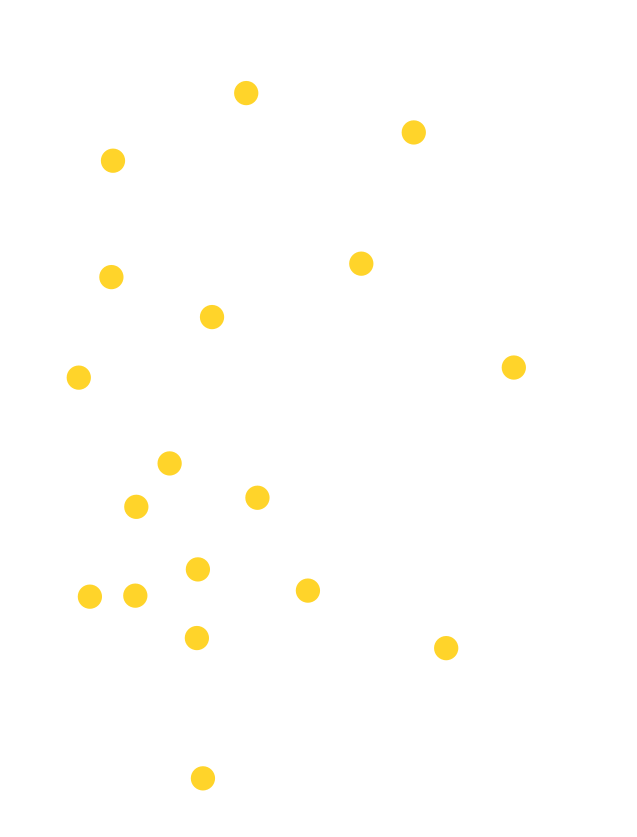
\includegraphics[width=0.3\linewidth]{figs/face-3d}
    \caption{Fitting a 3D model onto a 2D face}
    \label{}
\end{figure}

Once this is achieved, the translation and rotation of the 3D model (a
$4\times4$ transformation matrix) gives us an estimate of the real head pose of
the person \emph{relative to the camera}.

We actually do not need to fit (\emph{back-project}) many points of the 3D model
onto the 2D image to compute this transformation. Theoretically, 3 points are
enough. To make it more robust, we can however fit more points.

\begin{figure}[h!]
    \centering
    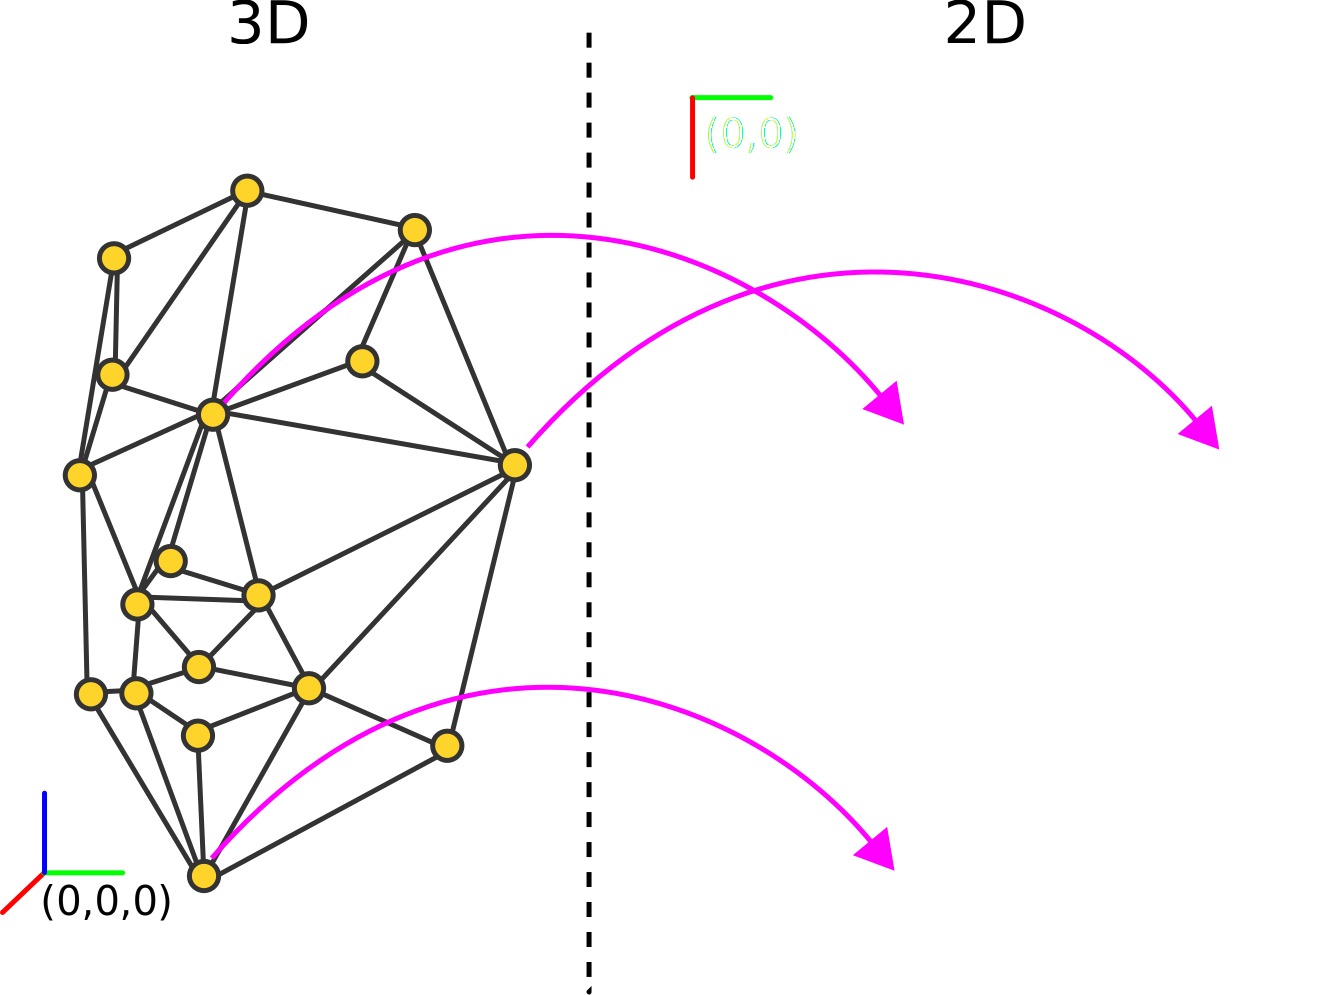
\includegraphics[width=0.6\linewidth]{figs/2d-3d}
    \caption{Establishing 2D-3D correspondances}
    \label{2d-3d}
\end{figure}

The \emph{fitting} operation is performed with the \emph{PnP} algorithm: it
takes 2D-3D correspondances (pairs of points: one on the 3D model and the
corresponding one in 2D, figure~\ref{2d-3d}) and iteratively computes the transformation that would
project the 3D points onto the corresponding 2D points.



\step{Choosing good correspondances}

The first step is to choose good pairs of 2D-3D points. Select 6 to 8 2D points
(take their IDs from figure~\ref{dlib-features}), and store the corresponding 3D
coordinates.

\begin{figure}[h!]
    \centering
    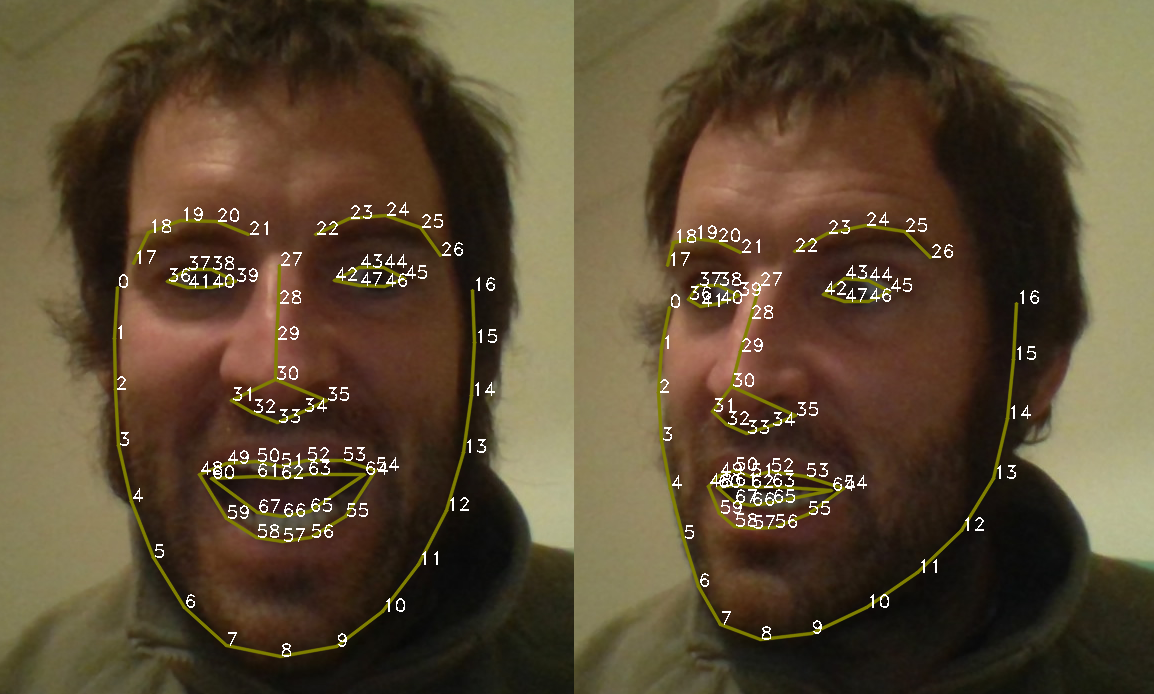
\includegraphics[width=0.9\linewidth]{figs/dlib-features}
    \caption{The 68 features detected by {\tt dlib}.}
    \label{dlib-features}
\end{figure}

To find the 3D coordinates, decide of an origin on the face (for instance, the
nose, or possibly better, the \emph{sellion} which lays between the two eyes),
and compute the position of the points relative to the nose. You can get the
anthropometry of an average adult head from figure~\ref{head} (that comes from
this wikipedia page: \url{https://en.wikipedia.org/wiki/Human_head}).

\begin{figure}[h!]
    \centering
    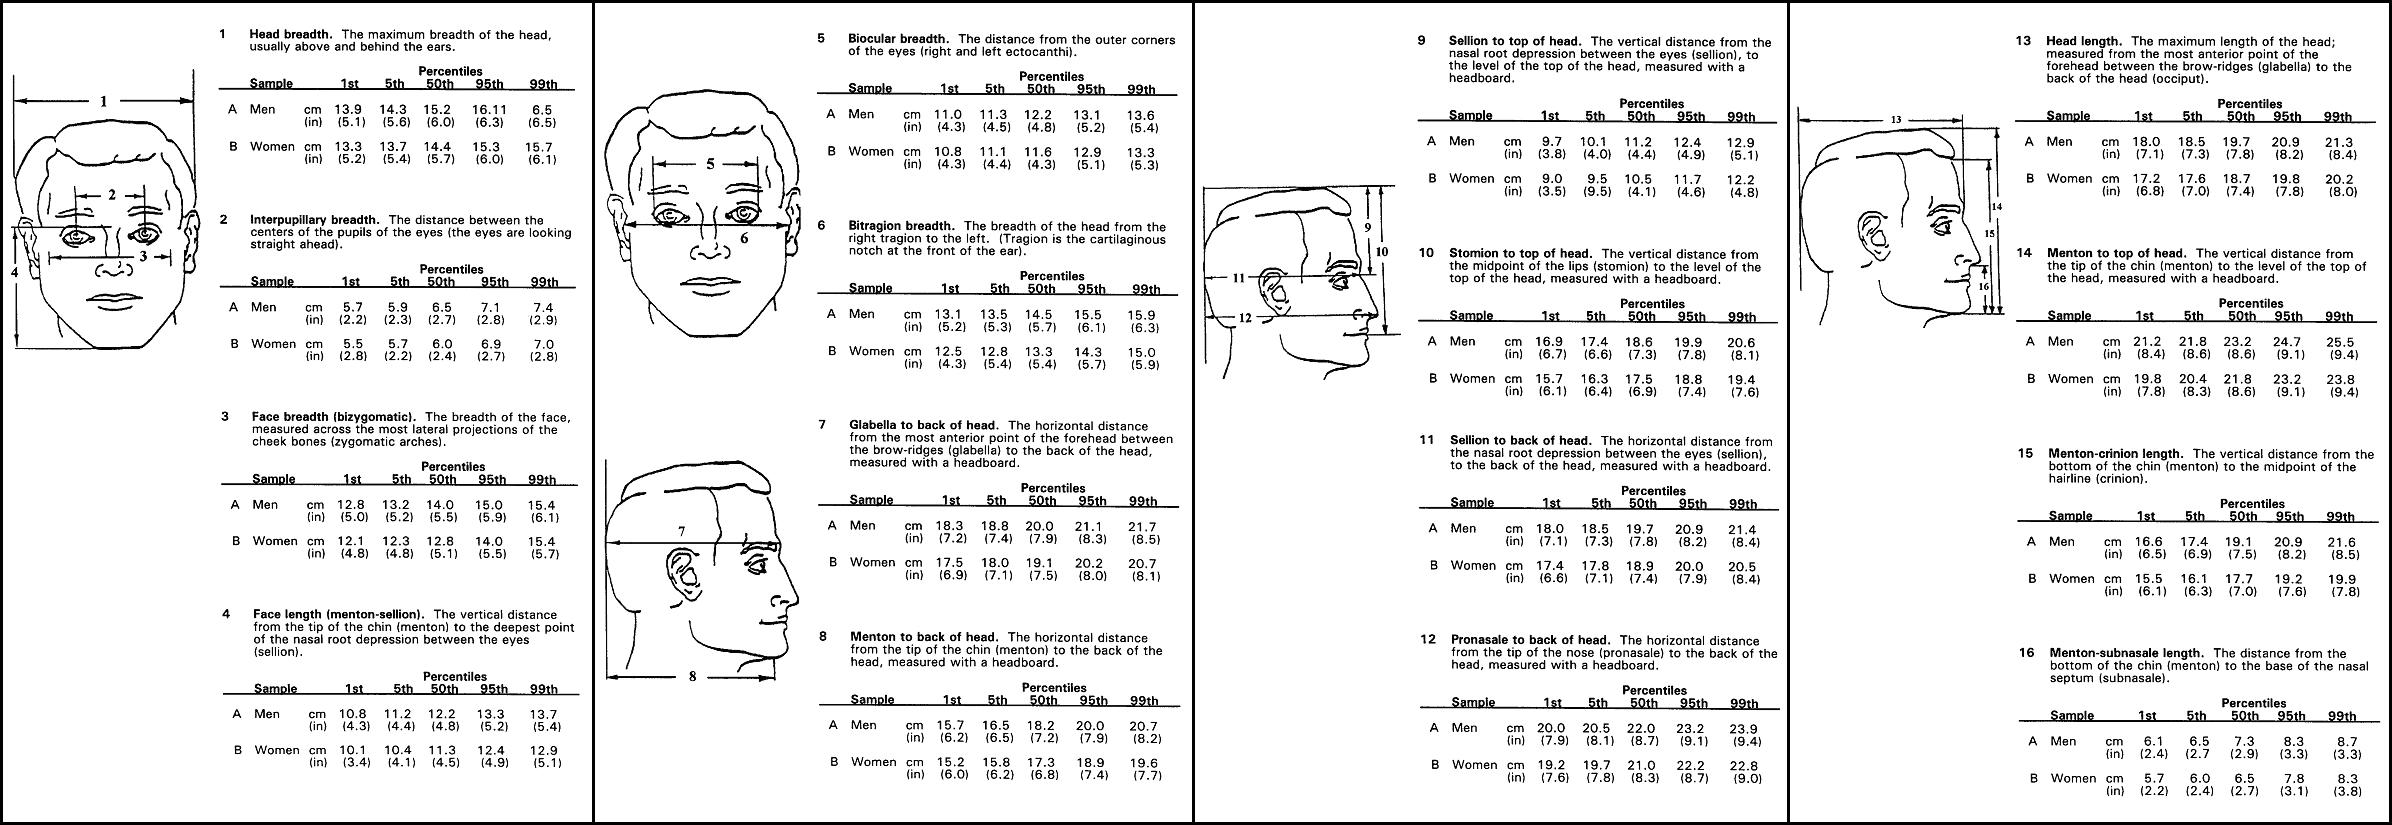
\includegraphics[width=1.\linewidth]{figs/headanthropometry}
    \caption{Adult human physical characteristics of the head.}
    \label{head}
\end{figure}

\note{Set X pointing forward and Z pointing up. Use millimeters.}

You can simply store them in the library header ({\tt
head\_pose\_estimation.hpp}) as respectively an enumaration and constants:

\begin{cppcode}
// Facial features index of interesting points
enum FACIAL_FEATURE {
    NOSE=30,
    RIGHT_EYE=36,
    LEFT_EYE=45,
    // Complete that!
};

// 3D coordinates of these points, assuming here that the nose is the origin
const static cv::Point3f NOSE_3D(0., 0., 0.);
const static cv::Point3f RIGHT_EYE_3D(-41., -65.5, 43.);
// Complete that!
\end{cppcode}



\step{From 2D to 3D: back-projection with solvePnP}

OpenCV's {\tt solvePnP} method implements the PnP algorithm.

To call it, you need to pass:
\begin{itemize}
    \item a vector of 3D points
    \item a vector of the corresponding 2D points
    \item and a projection matrix
\end{itemize}

Using the code provided below, modify {\tt src/head\_pose\_estimation.cpp} to
create a new method \\ \cpp{cv::Matx44d HeadPoseEstimation::pose(size_t face_idx)} that takes
the index of one of the detected faces, call \cpp{cv::solvePnP} from it, and
finally returns the transformation:

\begin{cppcode}

cv::Matx44d HeadPoseEstimation::pose(size_t face_idx)
{

    // Very simple projection matrix: we hardcode the focal length
    // to a reasonable value for webcams and the optical center is
    // simply the center of a 640x480px image.
    cv::Mat projectionMat = cv::Mat::zeros(3,3,CV_32F);
    cv::Matx33f projection = projectionMat;
    projection(0,0) = 500; // focal length (x)
    projection(1,1) = 500; // focal length (y)
    projection(0,2) = 320; // optical center (x)
    projection(1,2) = 240; // optical center (y)
    projection(2,2) = 1;

    std::vector<Point3f> head_points_3d;

    // TODO: fill the vector

    std::vector<Point2f> head_points_2d;

    // TODO: fill the vector

    Mat rvec, tvec;

    // TODO: call solvePnP to find the 3D pose of our head

    // transforms the rotation vector rvec into a rotation matrix
    Matx33d rotation;
    Rodrigues(rvec, rotation);


    // create the 4x4 transformation matrix (using meters for the translations)
    Matx44d pose = {
        rotation(0,0),    rotation(0,1),    rotation(0,2),    tvec.at<double>(0)/1000,
        rotation(1,0),    rotation(1,1),    rotation(1,2),    tvec.at<double>(1)/1000,
        rotation(2,0),    rotation(2,1),    rotation(2,2),    tvec.at<double>(2)/1000,
                    0,                0,                0,                          1
    };

    return pose;
}

/** Small helper method to extract the 2D coordinates of a facial feature
 */
Point2f HeadPoseEstimation::coordsOf(size_t face_idx, FACIAL_FEATURE feature)
{
    return toCv(shapes[face_idx].part(feature));
}

\end{cppcode}

\step{Display the head pose}

Using the provided code, overlay the 3 unit vectors X, Y, Z on top of the face
to show the 3D head pose.

\begin{cppcode}
// creates the 3 unit vectors
std::vector<Point3f> axes;
axes.push_back(Point3f(0,0,0));
axes.push_back(Point3f(50,0,0));
axes.push_back(Point3f(0,50,0));
axes.push_back(Point3f(0,0,50));
std::vector<Point2f> projected_axes;

// the opposite of solvePnP: it simply projects 3D points onto a 2D plan
// Use here the rvec and tvec returned by solvePnP
projectPoints(axes, rvec, tvec, projection, noArray(), projected_axes);

// displays the vectors as well as the coordinates
line(_debug, projected_axes[0], projected_axes[3], Scalar(255,0,0),2,CV_AA);
line(_debug, projected_axes[0], projected_axes[2], Scalar(0,255,0),2,CV_AA);
line(_debug, projected_axes[0], projected_axes[1], Scalar(0,0,255),2,CV_AA);

putText(_debug, "(" + to_string(int(pose(0,3) * 100)) + "cm, " 
                    + to_string(int(pose(1,3) * 100)) + "cm, " 
                    + to_string(int(pose(2,3) * 100)) + "cm)", 
        coordsOf(face_idx, NOSE), 
        FONT_HERSHEY_DUPLEX, 0.5, Scalar(0,0,255),2);

\end{cppcode}

Modify {\tt head\_detection.cpp} to call \cpp{HeadPoseEstimation::pose}.


\begin{figure}[h!]
    \centering
    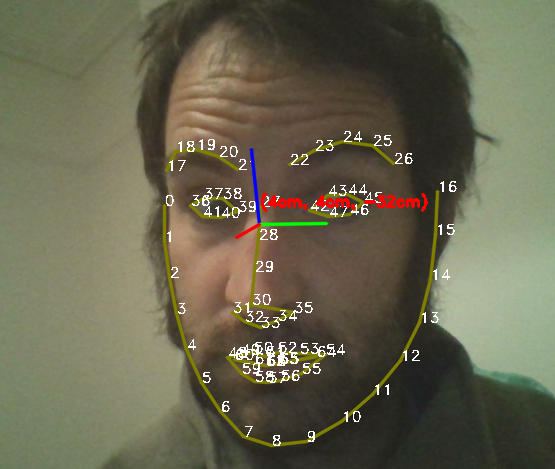
\includegraphics[width=0.6\linewidth]{figs/head_pose}
    \caption{Estimated head pose}
    \label{head_pose}
\end{figure}

You should now obtain something similar to figure~\ref{head_pose}. We have
estimated in real-time the 6D pose of the head using a monocular camera,
in about 100 lines of code, and this even works with multiple persons at the same
time. Not bad!

\part{Field of attention}

\step{Publishing the head pose as a {\it tf} frame}

The first step of the second part is to ``ROSify'' the head pose estimation: in
our case, it means publishing the head pose as a {\it tf} frame.

Start by copying the templates from {\tt templates/part2} to {\tt src/}, compile
them, and \textbf{install} them.

\begin{shcode}
$ cd $PROJECT_ROOT
$ cp -R templates/part2/* .
$ cd build
$ make && make install
\end{shcode}

If ROS is correctly set-up on your system, you should be able to launch the {\tt
head\_pose\_estimator} ROS node with:

\begin{shcode}
$ roslaunch attention_assessment attention_assessment.launch
\end{shcode}

\note{
    The {\tt head\_pose\_estimator} node needs a video stream as input. If you
    look at the launch file ({\tt attention\_assessment.launch}), you see that
    the launch file tries to launch {\tt gscam}. This node allows to stream the
    webcam or movies as a ROS image topic. Please download and install {\tt
    gscam} from \url{https://github.com/ros-drivers/gscam}. Note that this node
    relies on GStreamer: on Ubuntu, you need to install the package {\tt
    libgstreamer-plugins-base0.10-dev}.
}


Once you are able to run the node, complete it to actually broadcast one {\it
tf} frame per detected face.

You can use the following code to convert a \cpp{cv::Matx44d} transformation
matrix as returned by \cpp{HeadPoseEstimation::pose} into a
\cpp{tf::StampedTransform}:

\begin{cppcode}

// we assume 'face_idx' to be the index of the currently processed face, and
// 'pose' the corresponding 4x4 transformation matrix

tf::Transform face_pose;

// the frame orientation of the camera follows the classical camera
// convention (Z forward)
auto z = -pose(2,3);

face_pose.setOrigin(tf::Vector3(pose(0,3),
                                pose(1,3),
                                z) );

tf::Quaternion qrot;
tf::Matrix3x3 mrot(
        pose(0,0), pose(0,1), pose(0,2),
        pose(1,0), pose(1,1), pose(1,2),
        pose(2,0), pose(2,1), pose(2,2));
mrot.getRotation(qrot);
face_pose.setRotation(qrot);

auto tf_pose = tf::StampedTransform(face_pose, 
                                    ros::Time::now(), 
                                    cameraFrame,
                                    "face_" + to_string(face_idx)));
\end{cppcode}

\begin{figure}[h!]
    \centering
    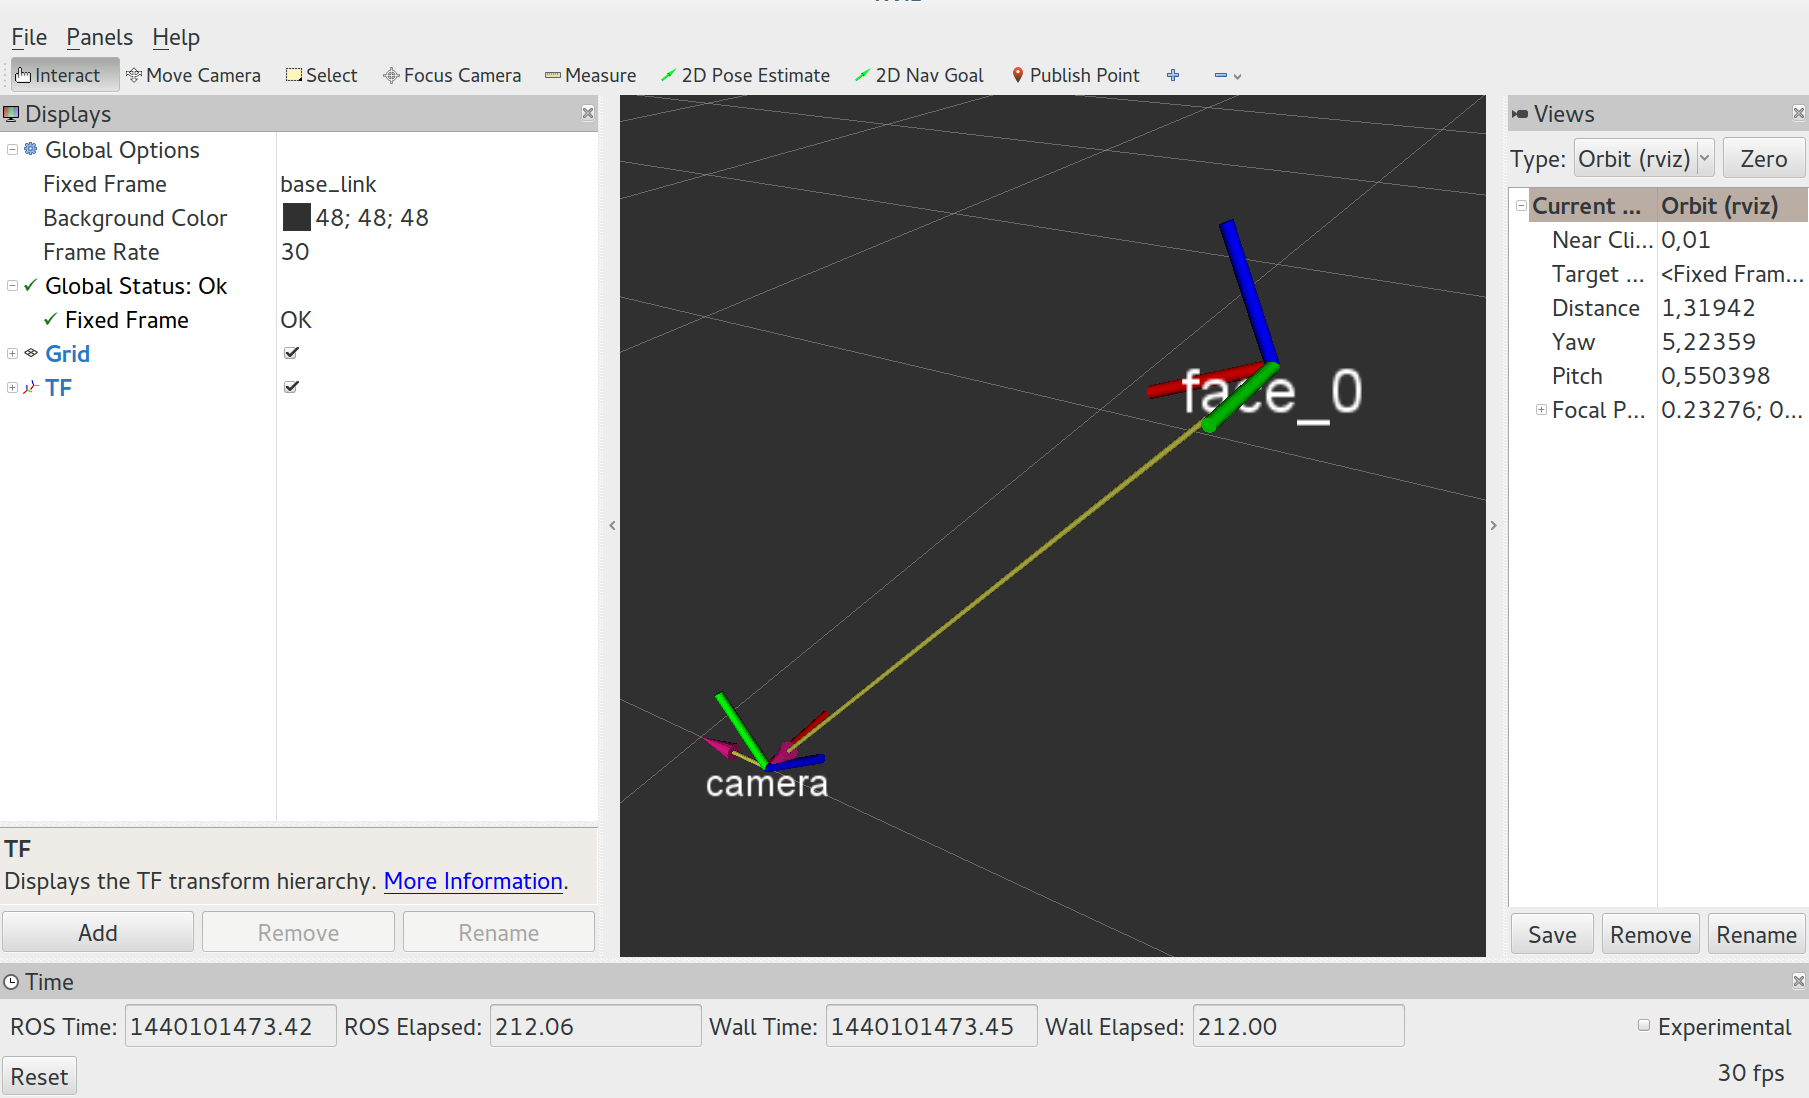
\includegraphics[width=0.9\linewidth]{figs/rviz}
    \caption{Screenshot of RViz displaying the 6D
    pose of a single face.}
    \label{rviz}
\end{figure}

Once complete, launch your node and start RViz. You should see something similar
to figure~\ref{rviz}.


\step{Visualization of the field of view and field of attention}

The next step consists in computing the field of view ({\it FoV}) and field of
attention ({\it FoA}) of the person. We model them as cones spanning from the
head's origin.

\important{This is a simplified model: obviously, one may move his/her eye balls --
    hence rotating the field of view -- without moving the head. However, this
    approximation work well enough in many situation. For a more accurate
    measurement of the direction of the field of view, one may resort to
    eye-tracking techniques.  }

\note{From now on, we will only consider the {\bf first} detected person,
    corresponding to the frame {\tt face\_0}. Support for multiple people is
    left as an exercise to the reader :-)}

A convenient way to represent the fields of view and fields of attention in RViz
is to simulate a range sensor, which is displayed in RViz as a cone.

Modify {\tt ros\_node.cpp} to publish the
fields of view and field of attention as range sensors, and check you can see
them in RViz (figure~\ref{fov}).

\begin{figure}
    \centering
    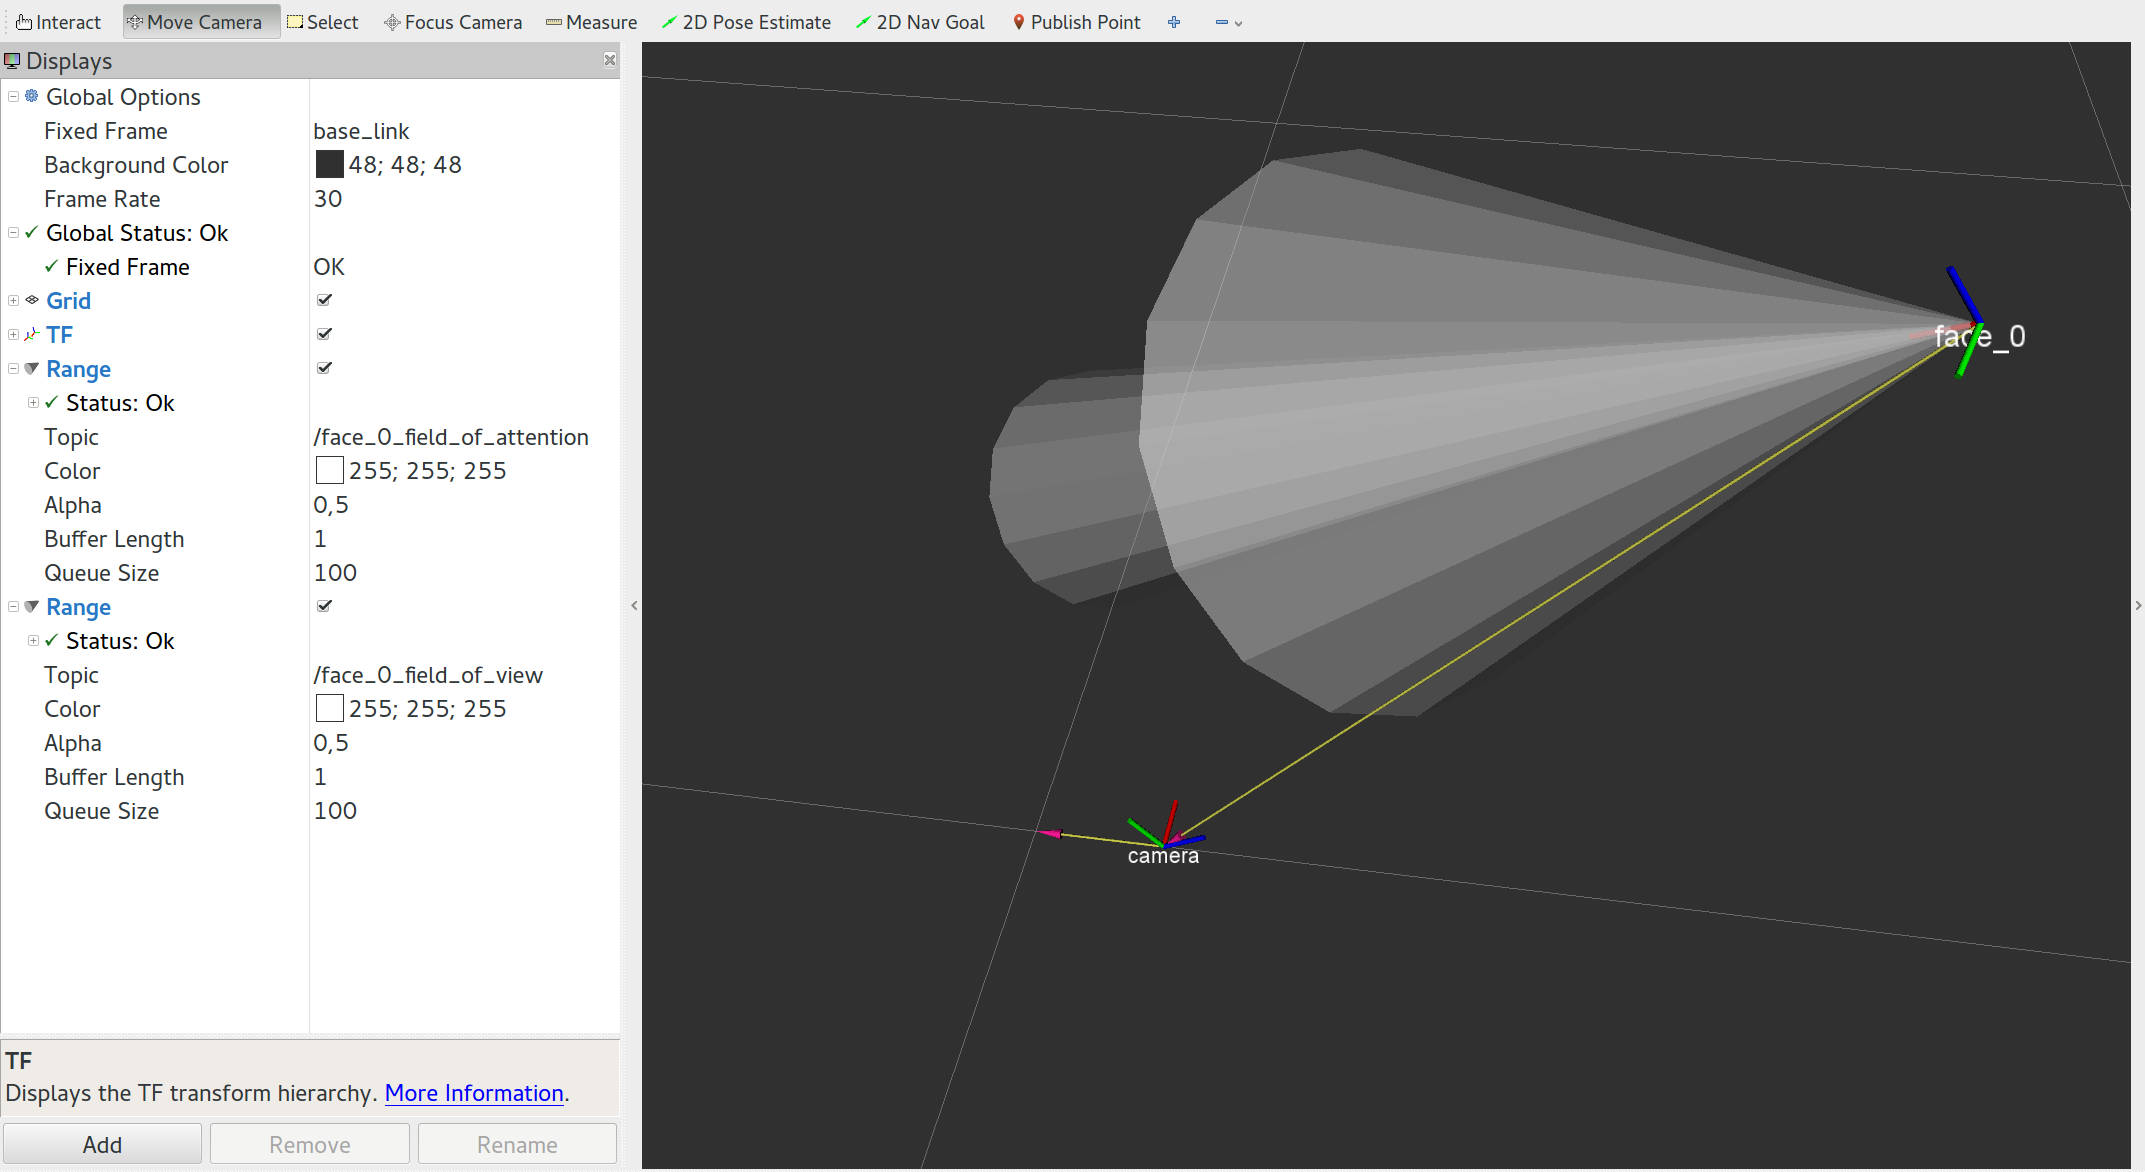
\includegraphics[width=0.9\linewidth]{figs/fov}
    \caption{Fields of view (large) and attention (narrow) displayed in RViz.}
    \label{fov}
\end{figure}

You can use the following code snippets to create the publishers (one for the
field of view, one for the field of attention) and to actually publish the range
sensor messages:

\begin{cppcode}
// To be added to the node's constructor. Do not forget to add the required
// declarations in the ros_node.hpp header

// Initialization of the FoV and FoA messages and publishing
fov_pub = rosNode.advertise<sensor_msgs::Range>("face_0_field_of_view", 1);
foa_pub = rosNode.advertise<sensor_msgs::Range>("face_0_field_of_attention", 1);

// the Range messages are actually almost constant! We can define them in the
// constructor.
fov.radiation_type = sensor_msgs::Range::INFRARED;
fov.field_of_view = 50. / 180 * M_PI; // radians
fov.min_range = 0;
fov.max_range = 10;
fov.range = 0.5; // meters

foa.radiation_type = sensor_msgs::Range::INFRARED;
foa.field_of_view = 15. / 180 * M_PI; // radians
foa.min_range = 0;
foa.max_range = 10;
foa.range = 1; // meters
\end{cppcode}

\begin{cppcode}
// To be added to the main loop

fov.header.stamp = ros::Time::now();
fov.header.frame_id = "face_0";
fov_pub.publish(fov); 

foa.header.stamp = ros::Time::now();
foa.header.frame_id = "face_0";
foa_pub.publish(foa); 
\end{cppcode}


\step{Who is in the field of attention?}

The next step consists in computing who/what is in the field of attention of the
person. It simply requires to compute which {\it tf} frames are within the field
of attention.

We implement this computation as a new, independent ROS node, written in Python.

Copy the provided Python template to create a new ROS node:

\begin{shcode}
$ cd $PROJECT_ROOT
$ cp -R templates/part2-python .
$ cd build
$ make install
\end{shcode}

This adds a new node called {\tt current\_focus}. It has been added to the
launch file, so start it by simply calling:

\begin{shcode}
$ roslaunch attention_assessment attention_assessment.launch
\end{shcode}

It does not do anything useful for now: complete it to publish on the topic {\tt
current\_focus} the list of {\it tf} frames that are currently in field of
attention of the person.

\part{Attention assessment}

\step{Plotting attention focus}

Copy the following Python template for a new ROS node that listen to {\tt
current\_focus} and plot in real-time the current focus(es):

\begin{shcode}
$ cd $PROJECT_ROOT
$ cp -R templates/part3-python .
$ cd build
$ make install
\end{shcode}

\note{This node requires {\tt matplotlib}. Install the package {\tt
python-matplotlib} if you do not have it yet.}

\begin{figure}[h!]
    \centering
    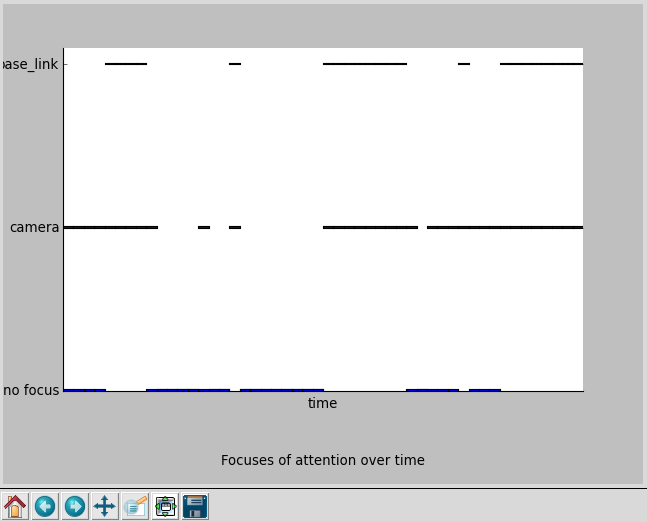
\includegraphics[width=0.6\linewidth]{figs/fov_plot}
    \caption{Focuses of attention over time: the lines indicate when the person
    was looking onto each of the frames.}
    \label{plot_focus}
\end{figure}

Complete the node {\tt focus\_analysis.py} as needed to plot the frames currently
on focus. When running this node, it should look similar to figure~\ref{plot_focus}.


\step{Real-world setup}

In a typical experiment, with one or several tasks at hand, the focus of
attention is expected to change over time.

To estimate if the user is currently engaged into the task, we therefore need to
compare, at a given time, if the current focus of attention matches the {\it
expected} focus of attention.

Figure~\ref{focuses} represents an example of a child-robot face-to-face
interaction. Depending on the phase of the interaction, the child would have to
look either to the robot, to one of the tablets, or to the experimenter. The
different possible focuses are depicted in red.

\begin{figure} [h!]
    \centering
    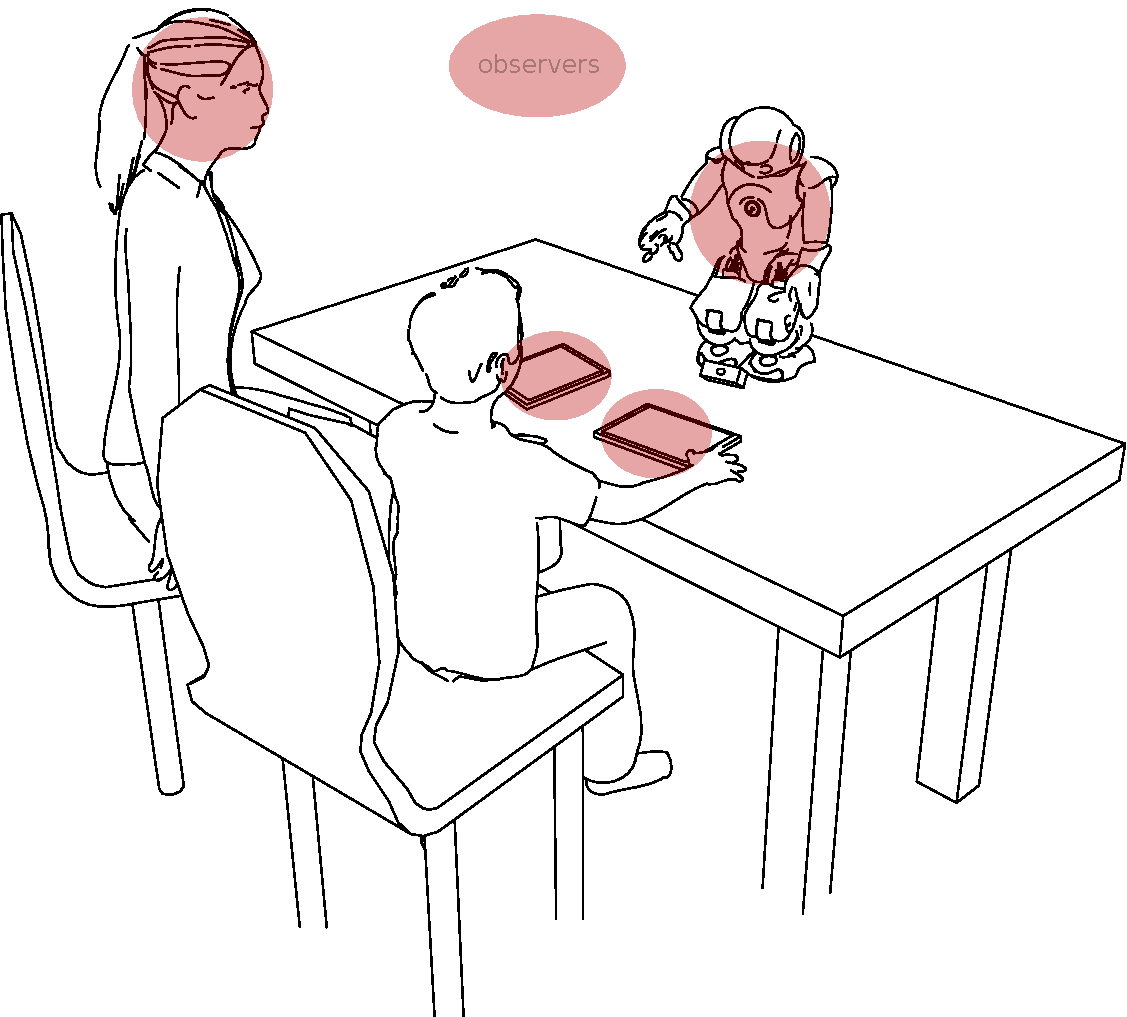
\includegraphics[width=0.7\linewidth]{figs/cowriter_setup}
    \caption{Typical child-robot face-to-face interaction. In red, the different
    possible focuses of attention: the expected current focus of the child
    changes over the task's duration.}
    \label{focuses}
\end{figure}

Using a real recorded experiment and the log of that experiment (which provides
the expected focuses of attention over time), we will next try to assess the
level of attention of a child during an interaction with a robot.

Figure~\ref{focuses} represents the experimental setup. We will assume that the
tablets, the robot and the experimenter did not move during the experiment.

First, we need to publish all the useful frames. Open {\tt
launch/attention\_assement.launch} and edit it to publish the following static
frames:

\begin{xmlcode}
<node name="tablet_transform" pkg="tf" type="static_transform_publisher" 
                                                args="0.3 0 0 0 0 0 /base_link /tablet 100"/>
<node name="selection_tablet_transform" pkg="tf" type="static_transform_publisher"
                                   args="0.3 -0.3 0 0 0 0 /base_link /selection_tablet 100"/>
<node name="experimenter_transform" pkg="tf" type="static_transform_publisher"
                                       args="0.5 -1 0.7 0 0 0 /base_link /experimenter 100"/>
<node name="observers_transform" pkg="tf" type="static_transform_publisher"
                                        args="-2.7 -0.5 0.7 0 0 0 /base_link /observer 100"/>
<node name="base_link_transform" pkg="tf" type="static_transform_publisher"
                                                     args="0 0 0 0 0 0 /map /base_link 100"/>
<node name="robot_transform" pkg="tf" type="static_transform_publisher" 
                                            args="0 0 0.5 0 0 0 /base_link /robot_head 100"/>
\end{xmlcode}

Test that the focus tracking and plotting works well with this more complex
environment.

Then, download the video from \url{http://goo.gl/KmA2Qn} (4.4MB), and modify the {\tt gscam}
invokation in the launch file to open it instead of the webcam:

\begin{xmlcode}
    <param name="gscam_config"
      value="filesrc location=<video path> ! decodebin2 name=dec ! queue ! ffmpegcolorspace"/>
\end{xmlcode}

Run again the project: this time, the head pose of the child on the video should
be tracked and his focus of attention should be plotted.

\note{If you want to see the video stream to ensure the head is correctly
tracked, either modify {\tt head\_detection.cpp} to open the vide instead of the
webcam, or modify the head pose estimation library to display the image. For
instance, adding
\cpp{imshow("headdetection", _debug);waitKey(10);} at the end of
\cpp{HeadPoseEstimation::update} in {\tt head\_pose\_estimation.cpp} will do.}

\step{Expected focus of attention}

To assess the engagement of the user in the interaction, we want to compare the
actual focuses of attention to the expected ones.

The file {\tt share/interaction.log} contains a simplified interaction log,
similar to what could be produced by the robot's execution manager.

The file {\tt nodes/log\_parsing.py} contains two functions to parse this log
file and convert it to a dictionary associating the expected focuses of
attention with their times.

If you run it, it should prints in 'real-time' the expected focus of attention.

\begin{shcode}
$ cd $PROJECT_ROOT/nodes
$ python log_parsing.py
\end{shcode}

Adapt {\tt focus\_analysis.py} to read the log file in parallel to the child's measured
focus. Create a new line on the plot that indicates when the \emph{expected
focus} and the \emph{actual focus} match.
%Figure~\ref{match} shows the result.
%
%\begin{figure}[h!]
%    \centering
%    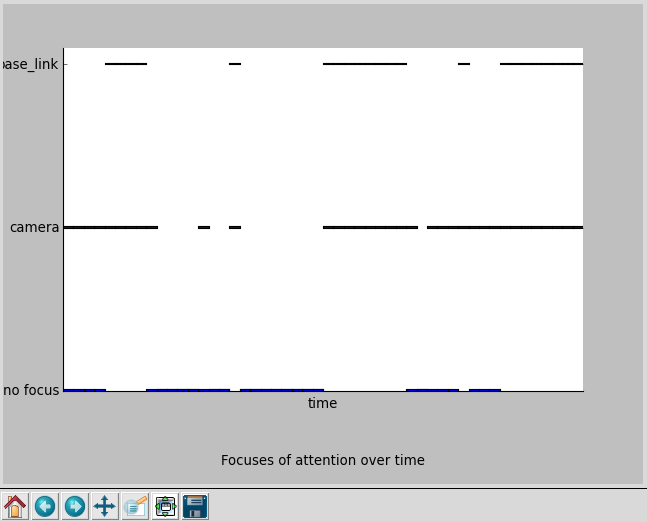
\includegraphics[width=0.6\linewidth]{figs/fov_plot}
%    \caption{TODO In red, the time period where the expected and actual focuses of
%    attention matched.}
%    \label{match}
%\end{figure}
%
\step{Level of attention}

Finally, compute a (naive) level of attention by incrementing a variable at
every step if the expected/actual focuses match, and decrementing it otherwise.
Plot it along the other values.

%\begin{figure}[h!]
%    \centering
%    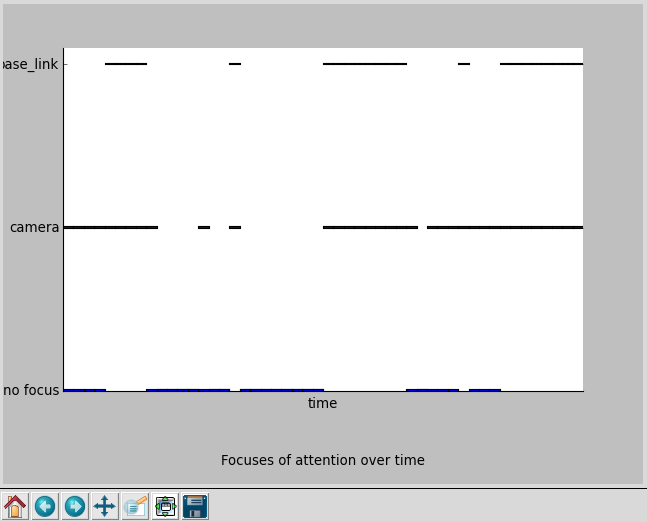
\includegraphics[width=0.6\linewidth]{figs/fov_plot}
%    \caption{TODO In blue, the naive yet real-time level of attention of the
%    child.}
%\end{figure}


%\part{Evaluating the assessment quality}

%\step{Inter-judge agreement}

\end{document}
